\subsection{IRNet}

% https://www.arxiv-vanity.com/papers/2208.04415/#S1.p3t

In Text-to-SQL tasks, the Intermediate Representation Network (IRNet)\cite{DBLP:journals/corr/abs-1905-08205} addresses two main challenges.
Among the challenges are mismatches between natural language intents and predicting columns resulting from a more significant number of out-of-domain words.
Instead of synthesizing SQL queries end-to-end, IRNet decomposes natural language into three phases (NL encoder, a schema encoder and a decoder).
Schema linking is performed over a database schema and a question during the first phase.
IRNet uses SemQL to bridge the gap between SQL and natural language.
It includes a Natural Language (NL) encoder, a Schema Encoder, and a Decoder.

\textbf{SemQL(Semantic Query Language)}\cite{semql}  is a query language designed explicitly for text-to-SQL tasks. It is a simplified version of SQL that is more human-readable and intuitive, making it easier for a model to generate SQL queries from natural language input. SemQL can be adapted to operate with various databases, letting users query whatever data source they need. This makes SemQL a flawless language for data-driven applications and analytics.

% add semql image
\begin{figure}[htb]
    \centering
    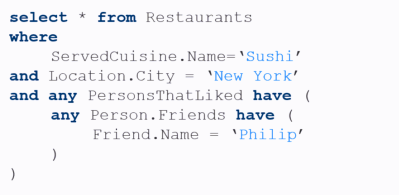
\includegraphics[width=0.4\textwidth]{pics/semql}
    \caption{SemQL query example\cite{2018MDM}}
    \label{fig:semql}
\end{figure}

% \begin{figure}[htb]
%     \centering
%     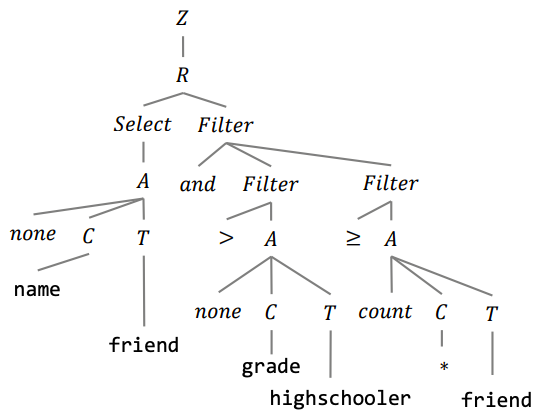
\includegraphics[width=0.5\textwidth]{pics/IRNet/illustrative_SemSQL}
%     \caption{An illustrative example of SemSQL from \cite{DBLP:journals/corr/abs-1905-08205}}
%     \label{fig:illustrative_SemSQL}
% \end{figure}


The IRNet model provides different functions to accomplish Text-to-SQL tasks.
Natural language is encoded into an embedding vector by the NL encoder. By using a bi-directional LSTM, these embedding vectors are used to construct hidden states.
A schema encoder takes a database schema as input and outputs representations for columns and tables.
Using context-free grammar, the decoder synthesizes SemQL queries.

\begin{figure}[htb]
    \centering
    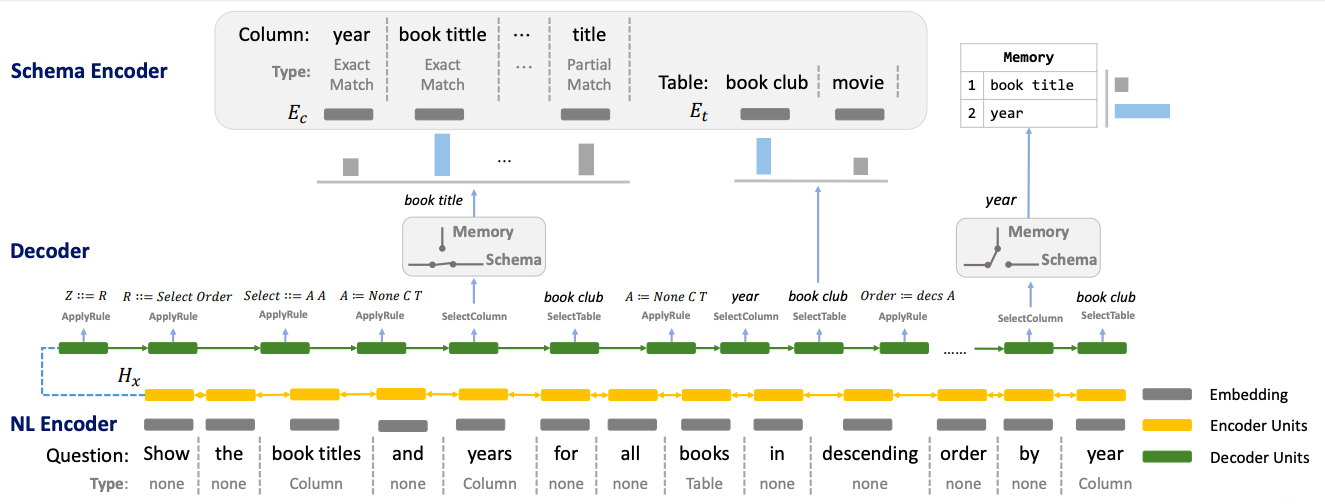
\includegraphics[width=1\textwidth]{pics/IRNet/overview}
    \caption{An overview of the neural model to synthesize SemQL queries\cite{DBLP:journals/corr/abs-1905-08205}}
    \label{fig:overview}
\end{figure}

They leverage BERT (Devlin et al., 2018) to encode questions, database schemas, and schema-linking results. The decoder stays the same. Notably, the sequence of spans in the question is concatenated with all the different column names in the schema. Each column name is divided with a unique token [SEP]. BERT takes the concatenation as input.

On the SPIDER dataset, IRNet performs 46.7\% better than previous benchmark models by 19\%. The accuracy of 54.7\% is achieved fine-tuneing BERT for IRNet.

\begin{figure}[htb]
    \centering
    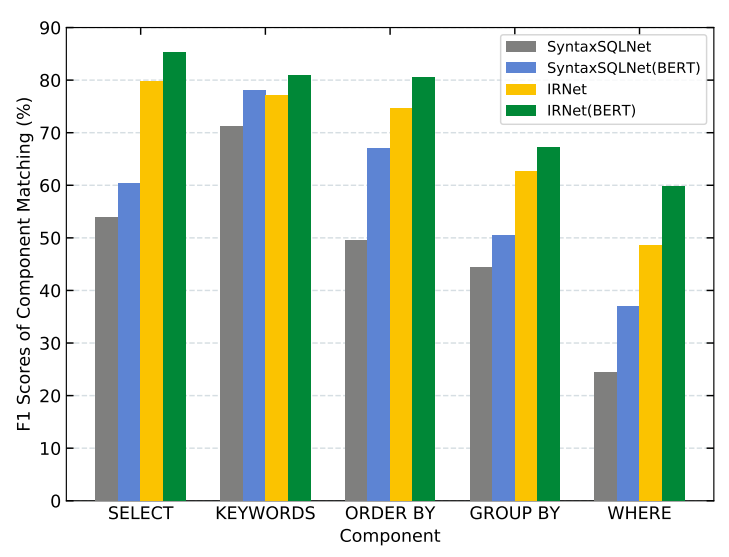
\includegraphics[width=0.6\textwidth]{pics/IRNet/f1}
    \caption{F1 scores of component matching of SyntaxSQLNet and IRNet on the test set from \cite{DBLP:journals/corr/abs-1905-08205}}
    \label{fig:f1}
\end{figure}
